\subsubsection{MOISE+}

O Moise+ é usado para realizar a especificação de sistemas multiagentes. Para cumprir com essa finalidade, existe três tipos de especificação que são; Estrutural, Funcional, e Deôntica. 

A especificação estrutural acontece em três níveis, individual, social e coletivo. O nível individual trata de definir os papeis $\rho$ dos agentes. Uma possível entre os papeis acontece por intermédio da hereditariedade em que se $\rho'$ é filho de $\rho$. Isso implica afirmar que $\rho'$ é uma especialização de $\rho$. Um exemplo apropriado para isso é o jogo de futebol onde existe o papel jogador dado por $\rho$ e existe o papel atacante dado por $\rho'$ \cite{mosieframework}. Em termos formais, essa relação é dada pro; 
\begin{eqnarray}\nonumber
\rho_a \sqsubset \rho_b
\end{eqnarray}

O nível social estabelece relações de ligação dado pelo predicado $link(\rho_s,\rho_d,t)$. Existe três possíveis valores para $t$, os quais são $t = \{aut, com, acq\}$. O valor $auth$ significa autoridade (neste caso $\rho_s$ exerce autoridade sobre $\rho_d$), o valor $com$ significa comunicação (neste caso $\rho_s$ pode se comunicar com $\rho_d$) e o valor $acq$ significa conhecimento ($\rho_s$ tem conhecimento da existência de $\rho_d$) \cite{mosieframework}. O MOISE+ define as seguintes relações de implicabilidade

\begin{eqnarray}\nonumber
	link(\rho_s,\rho_d,auth) \to link(\rho_s,\rho_d,com) \nonumber \\
	link(\rho_s,\rho_d,com) \to link(\rho_s,\rho_d,acq) 
\end{eqnarray}

O modelo também determina como se dá as relações de hereditariedade para o predicado de $link$, é dado por \cite{mosieframework}; 

\begin{eqnarray}\nonumber
	link(\rho_s,\rho_d,t) \wedge \rho_s' \sqsubset \rho_s' \to link(\rho_s',\rho_d,t) \nonumber \\
	link(\rho_s,\rho_d,t) \wedge \rho_d' \sqsubset \rho_d' \to link(\rho_s,\rho_d',t) 	
\end{eqnarray}


O nível coletivo determina a existência de compatibilidade entre os papeis \cite{mosieframework}. Essa é uma relação reflexiva e transitiva de determina que se um papel $\rho_a$ possui a capacidade de realizar um determinado objetivo, então o papel $\rho_b$ também tem essa capacidade. Em termos formais, essa relação se dá da seguinte forma \cite{mosieframework}.;

\begin{eqnarray}\nonumber
	\rho_a \bowtie \rho_b \wedge \rho_a \neq \rho_b \wedge \rho_a \sqsubset \rho' \to \rho' \bowtie \rho_b 
\end{eqnarray}

O nível coletivo também apresenta o conceito de grupo dado por $gt$ e constituído por;

\begin{eqnarray}\nonumber
	gt = \langle R,SG,L^{intra},L^{inter},C^{intra},C^{inter},np,ng\rangle 
\end{eqnarray}

Em que $R$ é o conjunto dos papeis não abstratos, $SG$ são subgrupos que estão contidos neste grupo, $L^{intra}$ consiste dos $links$ intra-grupos, $L^{inter}$ dos links inter-grupos, $C^{intra}$ das relações de compatibilidade intra-grupos e $C^{inter}$ das relações de compatibilidade inter-grupos. O símbolo $np$ denota a cardinalidade mínima e máxima para uma dada função e o símbolo $ng$ realiza o mesmo para os subgrupos \cite{mosieframework}. 

A Especificação Funcional tem como por finalidade descrever os objetivos a serem atingidos dentro de uma estrutura de árvore. A figura a seguir define como se dá esse tipo de especificação; 

\begin{figure}[H]
  \centering
  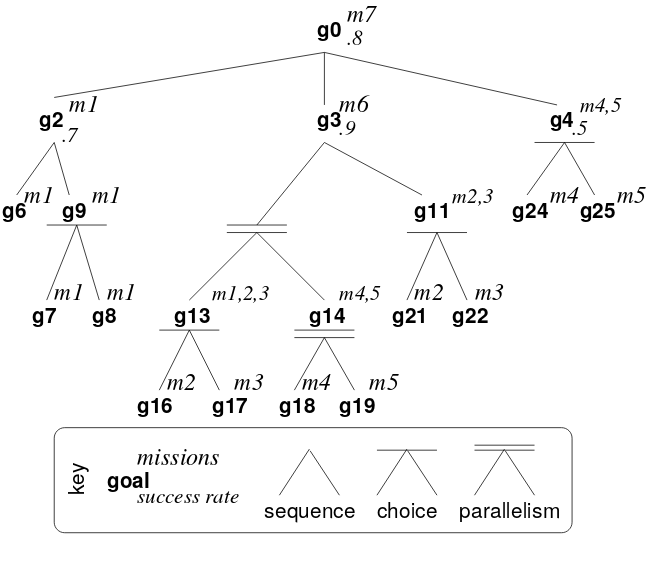
\includegraphics[width=0.8\linewidth]{figmoise} 
  \caption{Arvore de objetivos definido pelo modelo Moise \cite{mosieframework}}
  \label{arvoremoise}
\end{figure}

A figura \ref{arvoremoise} define três tipos de relação de subobjetivos; $sequence$ onde todos os subobjetivos devem necessariamente ser concluídos em sequência, $choice$ onde o agente tem a possibilidade de escolher qual objetivo ele deseja seguir e $parallelism$ onde todos os objetivos devem ser concluídos, contudo sem uma sequência definida. Como é possível observar na figura, os objetivos são agrupados em conjuntos de missões $m$. A relação a seguir define isso melhor;

\begin{eqnarray}\nonumber
	m_k = \{ g_n,...,g_m\}
\end{eqnarray}


A Especificação Deôntica define predicados para estabelecer permissões e obrigações entre os papeis e as missões. Toda obrigação implica necessariamente em uma permissão. A relação a seguir estabelece isso; 

\begin{eqnarray}\nonumber
	obl(\rho,m,tc) \to per(\rho,m,tc) \\
	obl(\rho,m,tc) \wedge \rho \sqsubset \rho' \to obl(\rho',m,tc) \\
	per(\rho,m,tc) \wedge \rho \sqsubset \rho' \to per(\rho',m,tc) \\	
\end{eqnarray}

Onde o predicado $obl$ define uma obrigação e o predicado $per$ define permissão. O argumento $tc$ define uma periodicidade de tempo para o qual a relação deôntica é valida. 

Existe muitos ponto similares entre o modelo proposto neste estudo e o Moise. Ambos os modelos apresentam papeis $\rho$, apresentam objetivos $g$ e apresentam relações deônticas de obrigação e permissão. Isso se deve ao fato, em partes, que o modelo proposto neste estudo importou muitos dos conceitos presentes no Moise tendo em vista a aplicabilidade para o domínio em interesse. Esses conceitos são importantes para o modelo deste estudo pois são grande relevância para descrever situações onde uma equipe de pessoas devem atingir certos objetivos trabalhando em cooperação. 

Contudo, ambos modelos apresentam diferenças significativas. Uma dessas diferenças reside em como as relações deônticas são atribuídas, pois no Moise a relação é feita entre o papel e a missão e no modelo proposto neste estudo a relação é feita entre o papel e o objetivo. Isso se deve ao fato de que uma das finalidades deste estudo consiste na realização de uma análise de sanções e violações. Como essas analises trabalham no nível de atividades, objetos e condições (dentro do contexto deste estudo), trabalhar na ordem de objetivos trás uma análise mais aprimorada no estudo das violações e sanções. 

O Moise não apresenta suporte a tratativa de sanções e violações. Assim sendo, para conseguir atingir um modelo onde fosse possível analisar certos tipos de sanções e violações de interesse, foi necessário introduzir predicados que não fazem parte do vocabulário e da sintaxe do Moise. 

O Moise trabalha uma estrutura lógica de interesse a descrição de grupos, \textit{links} e compatibilidades. Esses conceitos não são trabalhados no modelo em interesse por não serem necessários ao domínio de interesse deste estudo. Assim sendo, esses conceitos trariam complexidades adicionais sem justificativa válida para isso.
